\documentclass[specification,annotation]{itmo-student-thesis}

%% Опции пакета:
%% - specification - если есть, генерируется задание, иначе не генерируется
%% - annotation - если есть, генерируется аннотация, иначе не генерируется
%% - times - делает все шрифтом Times New Roman, требует пакета pscyr.

%% Делает запятую в формулах более интеллектуальной, например: 
%% $1,5x$ будет читаться как полтора икса, а не один запятая пять иксов. 
%% Однако если написать $1, 5x$, то все будет как прежде.
\usepackage{icomma}

\usepackage{float}

%% Данные пакеты необязательны к использованию в бакалаврских/магистерских
%% Они нужны для иллюстративных целей
%% Начало
\usepackage{tikz} 
\usetikzlibrary{arrows}

%% Указываем файл с библиографией.
\addbibresource{bachelor-thesis.bib}

\begin{document}

\studygroup{M3438}
\title{Инструмент для анализа производительности программ написанных на C++}
\author{Немченко Евгений Дмитриевич}{Немченко Е. Д.}
\supervisor{Корнеев Георгий Александрович}{Корнеев Г.А.}{кандидат техн. наук}{доцент кафедры КТ}
\secretary{Павлова Оксана Николаевна}
\publishyear{2017}
%% Дата выдачи задания. Можно не указывать, тогда надо будет заполнить от руки.
\startdate{01}{сентября}{2016}
%% Срок сдачи студентом работы. Можно не указывать, тогда надо будет заполнить от руки.
\finishdate{31}{мая}{2017}
%% Дата защиты. Можно не указывать, тогда надо будет заполнить от руки.
% \defencedate{}{}{2017}

\addconsultant{Шахметов М. С.}{руководитель группы в ООО «Научно-Технический Центр ПРОТЕЙ»}
%\addconsultant{Беззубик В.В.}{без степени, без звания}

%% Задание
%%% Техническое задание и исходные данные к работе
\technicalspec{Разработать инструмент для сбора информации о времени работы каждой функции. Проанализировать полученную информацию и визуализировать ее в удобном виде для быстрого нахождения узких мест в программе.}

%%% Содержание выпускной квалификационной работы (перечень подлежащих разработке вопросов)
\plannedcontents{
\begin{enumerate}
	\item Обзор предметной области
    \item Описание способа решения проблемы
    \item Реализация инструмента для сбора информации о времени работы
    \item Реализация инструмента для визуализации собранной информации
\end{enumerate}
}

%%% Исходные материалы и пособия 
\plannedsources{\begin{enumerate}
	\item Susan L. Graham, Peter B. Kessler, and Marshall K. McKusick. 2004. gprof: a call graph execution profiler. SIGPLAN Not. 39, 4 (April 2004), 49-57. DOI=http://dx.doi.org/10.1145/989393.989401
    \item Jennifer M. Anderson, Lance M. Berc, Jeffrey Dean, Sanjay Ghemawat, Monika R. Henzinger, Shun-Tak A. Leung, Richard L. Sites, Mark T. Vandevoorde, Carl A. Waldspurger, and William E. Weihl. 1997. Continuous profiling: where have all the cycles gone?. ACM Trans. Comput. Syst. 15, 4 (November 1997), 357-390. DOI=http://dx.doi.org/10.1145/265924.265925
    \item Gang Ren, Eric Tune, Tipp Moseley, Yixin Shi, Silvius Rus, and Robert Hundt. 2010. Google-Wide Profiling: A Continuous Profiling Infrastructure for Data Centers. IEEE Micro 30, 4 (July 2010), 65-79. DOI=http://dx.doi.org/10.1109/MM.2010.68
\end{enumerate}}

%%% Календарный план
\addstage{Ознакомление с предметной областью}{14.11.2016}
\addstage{Ознакомление с существующими решениями}{24.12.2016}
\addstage{Реализация инструмента для сбора информации о приложении}{10.02.2017}
\addstage{Реализация инструмента для визуализации}{30.03.2017}
\addstage{Дальнейшие исследования}{30.04.2017}
\addstage{Написание пояснительной записки}{15.05.2017}
\addstage{Доработка пояснительной записки}{31.05.2017}

%%% Цель исследования
\researchaim{Разработать инструмент для анализа производительности, позволяющий ускорить поиск узких мест в программах, работающих в реальном времени, на протяжении долгого периода.}

%%% Задачи, решаемые в ВКР
\researchtargets{\begin{enumerate}
    \item выполнять сбор информации о запущенном приложении
    \item визуализировать собранную информацию в удобном для анализа виде
\end{enumerate}}

%%% Использование современных пакетов компьютерных программ и технологий
\advancedtechnologyusage{Был использован язык программирования C++, POSIX API, фреймворк Qt, проект libunwind, интегрированная среда разработки Qt Creator, распределенная система управления версиями Mercurial, сервер для непрерывной интеграции TeamCity.}

%%% Краткая характеристика полученных результатов 
\researchsummary{В результате были написаны инструменты один из которых предназначен для сбора информации, позволяющий собирать стеки вызовов с других приложений. Также был написан графический интерфейс для отображения полученных данных в удобном для анализа виде.}

%%% Гранты, полученные при выполнении работы 
\researchfunding{Грантов или других форм государственной поддержи и субсидирования в процессе работы не предусматривалось.}

%%% Наличие публикаций и выступлений на конференциях по теме выпускной работы
\researchpublications{}

%% Эта команда генерирует титульный лист и аннотацию.
\maketitle{Бакалавр}

%% Оглавление
\tableofcontents

%-*-coding: utf-8-*-
%% Макрос для введения. Совместим со старым стилевиком.
\startprefacepage
	Основной целью данной работы является создания инструмента для ускорения процесса поиска \enquote{узких} мест в программах.  

	В современном мире все чаще внимание уделяется скорости работы программ. Пользователям важен быстрый ответ. Программы должны уметь справляться с обработкой большого, постоянно меняющегося, входного объема данных. Им нужно уметь обрабатывать все данные и совершать нужные действия в зависимости от них, пока не пришли новые. Если приложение перестает справляться с нагрузкой, то некоторые запросы не будут обработаны. Из-за чего ухудшается качество написанного продукта.

	Программы, которые анализируют поток интернет трафика, например DPI \cite{dpi}, очень сложно поддаются анализу и поиску критических мест стандартными средствами. Так например долго работающая программа в течении дня, может в короткий промежуток времени начать \enquote{тормозить}. Из-за чего она не успевает отвечать на новые запросы и происходят потери данных, которые были посланы на сетевую карту. Стандартные средства для анализа приложений написаны таким образом, чтобы использоваться для программ запущенных на короткое время и зачастую нужно им на вход передавать специальные данные, которые были бы показательными и могли привести к нахождению проблемных участков кода.

	Стандартные средства не подходят для  по нескольким причинам. Некоторый из них сильно замедляют работу, потому их нельзя запускать на реальном приложении. Некоторые могут привести программу в нерабочее состояние. По отчетам многих из них сложно понять, где в программе возникли проблемы. А также они считают время занимаемое каждой функции в среднем, за весь промежуток работы. Это не позволяет смотреть на состояние системы в фиксированные моменты времени.
    
    В связи с чем возникает задача написания своего инструмента для анализа производительности. Он должен уметь собирать информацию с приложения, а также отображать ее пользователям. Инструмент должен быть прост в использовании. Должна быть возможность смотреть состояние программы на определенный промежуток времени.  
    
    Написанный инструмент поможет выявить проблемные участки кода. Исправление которых ускорит приложение и поможет ему обрабатывать весь поток входящих данных без потерь.

	Первая глава работы посвящена обзору существующих решений. Там же обсуждаются проблемы текущих решений и формулируется постановка задачи. 

	Во второй главе будет рассмотрена архитектура инструмента по сбору информации о приложении. Трудности возникающие при его написании.

	В третьей главе будет показан инструмент для визуализации собранных данных и рассказаны основные моменты возникающие при его реализации.

В заключении  показано текущее состояния разработки и рассмотрены перспективы ее развития. 
%-*-coding: utf-8-*-

\chapter{Постановка задачи}

	В настоящее время, поиск \enquote{горячих} мест в программах завоевал достаточно широкую популярность. Многие компании, такие как Google, Yandex, Intel стараются писать приложения работающие как можно быстрее. Пользователи не готовы ждать, а улучшение производительности той или иной компоненты на долю процента, стоит огромных денег таким крупным игрокам на рынке. Особенно это важно компаниям работающих в сфере HFT \cite{hft}. В Google даже используют такую неформальную метрику \enquote{количество долларов за изменение в производительности кода} \cite{gwp}.

	В связи с чем возникает потребность в программе, которая бы помогала программистам искать узкие места в их приложениях. Сейчас существуют несколько решений и подходов к данной задачи. Все они не подошли по ряду причин, после чего было решено написать свой инструмент, который бы не имел недостатков, присущих в других решениях данной задачи.

\section{Термины и понятия}

	\textbf{Профилирование} - сбор характеристик работы программы, таких как время работы каждой функции данной программы. 
    
    \textbf{Профайлер} - программа которая занимается профилированием других приложений, предназначенная для сбора информации и визуализации полученных данных с целью поиска критических участков кода.
    
    \textbf{Профиль приложения} - информация о работе профилируемого приложения, собранная во время профилирования.
    
    \textbf{Стек вызовов} - упорядоченная последовательность адресов функций, которая привела программу в текущее состояние.
    
    \textbf{Сэмпл} - один из стеков вызовов полученный во время профилирования.
    
    \textbf{Сигнал} - UNIX сигнал, асинхронное уведомление, которое можно послать процессу или определенному потоку. Приводит к остановке работы текущей единицы исполнения и вызову обработчика сигнала.  
    
    \textbf{Символы} - символьная информация, хранящаяся в исполняемом файле. Например название функции находящейся по определенному адресу.
        
    \textbf{Деманглирование} - декодирование имени функции. 
    
    \textbf{Разрешение символов} - преобразование адресов программы в закодированные названия функций, которые после необходимо деманглировать.
    
    
    \textbf{Стековый кадр} - часть данных, которая сохраняется перед началом исполнения кода функции, например, старые значения регистров, чтобы не испортить их предыдущие значения.
        
    \textbf{tid} - идентификатор потока исполнения.
    
    \textbf{pid} - идентификатор процесса.


\section{Обзор существующих решений}

	На данный момент написано множество различных профайлеров. По своему типу они бывают:
    \begin{itemize}
    	\item На основе событий
        \item Статистические или сэмплирующие
        \item Инструментирующие код
    \end{itemize}
    
    \textbf{На основе событий} профайлеры обычно реагирует на происходящие изменения и в этот момент записывают соответствующую информацию. Например на вызов функции или выход из нее. 
    
    \textbf{Статистические или сэмплирующие} - собирают информацию о приложении через определенные интервалы времени, приостанавливая его работу на короткий промежуток времени. Зачастую такие профайлеры менее точны, но этого достаточно, чтобы обнаружить проблемные участки. Такие инструменты почти не замедляют работающее приложение. Также, зачастую, они не требуют наличия исходных кодов и перекомпиляции приложения, что значительно упрощают работу с ними.
    
    \textbf{Инструментирующие код} - такие профайлеры меняют исходный код программы, вставляя в нужном месте вызов своих функций для подсчета информации. Они зачастую привносят очень большие накладные расходы приложению. Ими сложнее воспользоваться, когда хочется профилировать уже скомпилированное приложение.
    
    Далее будут рассмотрены доступные в свободном доступе профайлеры под систему Linux:
    \begin{itemize}
    	\item gprof \cite{gprof}
        \item google-perftools  \cite{gperf}
        \item perf \cite{perf}
        \item OProfile \cite{oprofile}
        \item callgrind \cite{valgrind}
    \end{itemize}
    
    \textbf{gprof} - смесь инструментирующего профайлера и сэмплирующего. Инструментация кода происходит автоматически во время компиляции, в компилияторе \verb|gcc|, например, можно включить его опцией \verb|-pg|. Перед входом в каждую функцию вставляется вызов функции \verb|mcount|. Сэмплированные данные вместе с дополнительной информацией сохраняются в файл \verb|gmon.out| и могут быть проанализированы при помощи утилиты \verb|gprof|.
    
    У него присутствует множество проблем из-за которых возникают трудности в использовании. Инструментируя код, потенциально можно сильно замедлить приложение. Накладные рассходы на CPU могут быть 30\%-260\%. Возникает это, если маленькие функции, которые очень часто вызываются будут инструментированы, что может быть дольше чем выполнение самой функции. Во вторых он не умеет работать с не статической сборкой приложения. В связи с чем не отображается информация о времени работы функций из библиотек загруженных динамически, из-за чего происходит потеря важной информации. Также он не умеет показывать информацию по каждому потоку в отдельности, что очень важно при поиске узких мест.  А также нельзя смотреть состояние процесса на определенный момент времени.
    
    \textbf{google-perftools} - инструмент разработанный компанией Google для их внутренних нужд. Он отлично работает с приложениями скомпилированными не статически. Он является сэмплирующим, настраивает интервальный  системный таймер, по истечении которого процесс прерывается сигналом SIGPROF. После они разворачивают стек при помощи библиотеки libunwind. Так как это происходит в рамках того же процесса которое профилируется, может возникнуть следующиая ситуация. Если программа бросает исключение, во время раскрутки стека вызывается функция \verb|_Unwind_Find_FDE| библиотеки libunwind. Внутри себя она берет блокировку, если они прервали приложение в этот момент, то в обработчике сигнала они тоже вызывают эту функцию и попадают в deadlock. В итоге этот профайлер мы не можем запускать на реально работающих приложениях использующих исключения, из-за потенциальной возможности сломать его.
    
    \textbf{perf и OProfile} - одни из самых часто используемых инструментов на Linux \cite{ibm}. Они умеют подключаться к приложению по pid. Собирать с него информацию, привносят незаметные накладные расходы на приложение. Но также не подходят из-за невозможности видеть состояние системы в определенные промежутки времени в визуализаторах, отображающих собранную информациюй. Хотя временные метки могут быть записаны в файл.
    
    \textbf{Callgrind} - этот инструмент является частью проекта Valgrind \cite{valgrind}. Он запускается в структуре Valgrind. При использовании Callgrind профилируемый код трансформируется в промежуточный язык и запускается на виртуальном процессоре имитируемом Valgrind. Что влечет за собой большие накладные расходы, но качество профиля очень хорошее. Замедление, работающей программы, может варьироваться в пределах от 10 до 50 раз. Из-за больших накладных расходов мы не можем использовать его на реальных системах.
    
\section{Уточненные требования к работе}
	Актуальность создания своего инструмента была показана ранее. От нового ожидается увидеть возможность собирать стек вызовов не испортив профилируемое приложение. Например \verb|gperftools| может привести во взаимную блокировку профилируемое приложение во время сбора информации \cite{deadlock_gperf}, необходимо избежать таких ситуаций. Сбор в реальном времени не должен сильно замедлять работоспособность программы. Профайлер должен уметь собирать информацию со всех потоков, не вынуждая совершать пользователей каких-либо дополнительных усилий. Вся информация собранная в процессе профилирования должна быть аннотирована временными метками, для возможности дальнейшего исследования. Также профайлер должен сохранить информацию о текущем адресном пространстве приложения, для восстановления символов. Собранная информация на одной машине должна без проблем быть прочитана и восстановлена на другой. 
    
    Также должен  быть создан инструмент для визуализации собранных данных, с помощью которого можно было бы искать узкие места в программах. Должна присутствовать возможность смотреть состояние профилированной программы в определенные моменты времени.

\chapterconclusion
	В данной главе была поставлена задача. Приведены основные термины и понятие используемые в этой работе. Также было рассказано о способах решения данной проблемы и существующие решения. Как видно ни одно из них не умеет решать поставленной задачи. В связи с чем возникает потребность в написании собственного инструмента.
    

%-*-coding: utf-8-*-
\chapter{Сбор информации о приложении}
	В данной главе будут описаны подходы к решению задачи сбора информации о приложении. Также будут рассмотрены основные аспекты и сложности возникающие при ее решении. В конце будет показан анализ накладных расходов на профилируемое приложение. 

\section{Общий принцип работы}
	На рисунке \ref{fig:general_profiler} можно увидеть алгоритм работы, детали которого будут описаны в следующих секциях. Профайлер способен работать в двух режимах: 

\begin{enumerate}
	\item запуская программу
    \item подключаться к уже запущенному приложению
\end{enumerate}

	В первом режиме профайлер сам запускает программу посредством функции \verb|execvp(...)| и контролирует ее время жизни. Если профайлер будет остановлен по требованию пользователя, то он также завершит и выполнение профилируемой программы.
    
    Во втором случае профайлеру нужны будут права супер пользователя. В системе Linux нельзя подключаться к другим приложениям не имея соответствующих прав. Профайлер собирает профиль приложения, до тех пор пока оно не завершится, либо не завершат сам профайлер. После профайлер отключается от приложения и оно продолжает работать как прежде.
    
    В обоих случаях, перед завершением работы, профайлер собирает символьную информацию с приложения. Так же символьную информацию необходимо собрать с библиотек и вся эта информация записывается в файл \verb|prof.pdb|. Параллельно с профилированием информация о текущей работе записывается в файл \verb|log.txt|, чтение которого может рассказать пользователю, как происходила работа во время профилирования.
    
    \begin{figure}[H]
        \caption{Общий принцип работы инструмента по сбору информации}
        \label{fig:general_profiler}
        \centering
        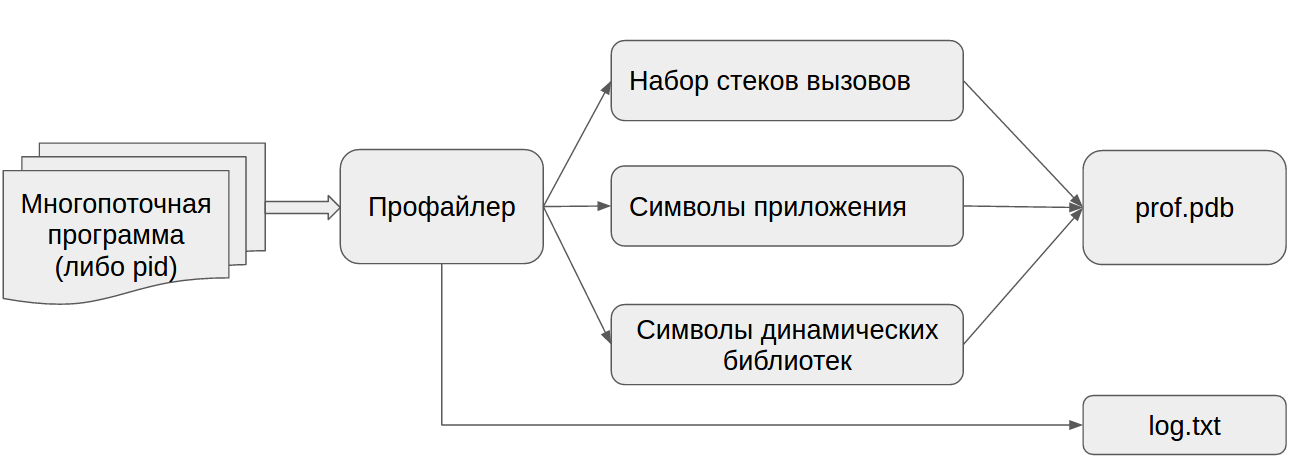
\includegraphics[width=\linewidth]{images/general_profiler}
    \end{figure}    
    
\section{Мониторинг запущенных потоков}
	Сбор стеков вызовов должен происходить для каждого потока отдельно, поэтому в этой секции будет рассказано про методы для мониторинга запущенных потоков. Если собирать всю информацию не выделяя каждый поток отдельно, получится перемешанная информация, которую сложно анализировать. Например, если пользователю интересны только некоторые из работающих потоков, ему будет удобнее посмотреть только на статистику внутри них, не показываю всю информацию о приложении. В языке C++ \cite{meyers} нет функции или простого способа для получения списка текущих потоков и мониторинга за ними. Далее будут показаны возможные решение их плюсы и недостатки.
    
    Для получения списка текущих потоков для приложения в Linux можно, например, перегрузив функцию \verb|pthread_create|. Так как она реализована в \verb|libpthread.so| можно подгрузить настоящую функцию при помощи \verb|dlopen| и заменить ее своей с добавлением \verb|tid| в специальный контейнер. С помощью этого можно мониторить создание потоков. Теперь только, чтобы подменить стандартную реализацию создания потоков на новую нужно скомпилировать ее как динамическую библиотеку. Пользователю для профилирования придется использовать подмену переменной окружения перед запуском \verb|LD_PRELOAD|, чтобы наша библиотека загрузилась раньше стандартной. Также данный подход не будет работать при статической сборке из-за этого он не подходит. Однако ровно так предлагают решить проблему с потоками в профайлере \verb|google-perftools|.
    
    Также можно воспользоваться утилитой \verb|ps| которая отображает текущие запущенные процессы и при помощи \verb|grep| найти нужные потоки. При использовании данного подхода было выявлено, что он очень медленно работает и сильно \enquote{тормозит} профайлер, так как список текущих потоков приходится брать каждый раз перед началом сбора стеков вызовов. 
    
    Третье решение наиболее удачно подошло для поставленной задачи. В Linux есть специальная файловая система \verb|procfs| которая представляет информацию о запущенных процессах. В разделе \verb|/proc/pid/task| можно найти информацию о всех потоках запущенных для данного pid. Сканируя данную директорию можно получить все необходимые идентификаторы потоков. Это приходится делать каждый раз перед сбором стеков вызовов, так как потоки могут завершаться и создаваться заново. По тестам проведенным в процессе написания профайлера было выявлено, что такой подход хорошо работает и почти не привносит дополнительных накладных расходов по сравнению с предыдущими.    
    
\section{Остановка потоков приложения}
	Чтобы развернуть стек вызовов для конкретного потока для начала нужно его остановить. Когда мы получили список идентификаторов всех потоков, нужно подключится к ним для возможности смотреть на их текущее состояние. Подключение к потокам осуществляется через системный вызов \verb|ptrace| при помощи \verb|PTRACE_ATTACH| иллюстрацию можно увидеть на рис. \ref{fig:ptrace_attach}. Подключившись к каждому потоку появляется возможность управлять его работой. Главный поток необходимо зарегистрировать на событие выхода при помощи \verb|PTRACE_SETOPTIONS|, чтобы профайлер узнал о том, что приложение собирается закрыться до того как оно очистило все свои ресурсы и выгрузило информацию о динамических библиотеках.
    
    \begin{figure}[H]
        \caption{Подключение к профилируемому приложению}
        \label{fig:ptrace_attach}
        \centering
        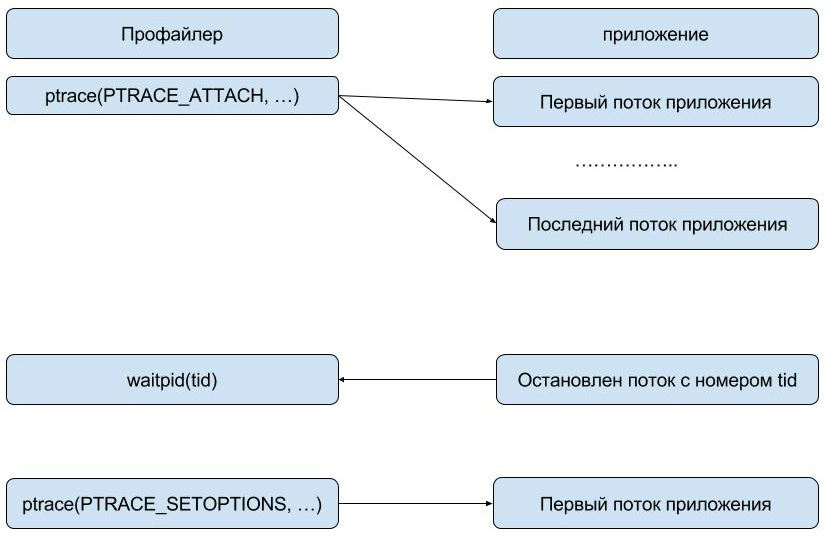
\includegraphics[width=\linewidth]{images/ptrace_attach}
    \end{figure}    
    
    Для остановки каждого потока используется отправка сигнала \verb|SIGSTOP| посредством системного вызова \verb|tkill|. Этот сигнал в системе Linux не может быть обработан или проигнорирован приложением. Он приостанавливает данный поток, после чего появляется возможность смотреть на его текущее состояние. Из-за того, что посылка сигнала происходит из другого приложения то он получается не мгновенно. Также поток может находится в очереди на исполнения, если их больше чем физических ядер. Поэтому сигнал может ему прийти не скоро и профайлер не должен останавливать свою работу из-за одного спящего потока. Для этого был реализован метод для асинхронной отправки сигнала и проверки, без ожидания, состояния всех потоков. В тот момент когда сигнал дойдет и поток действительно остановится можно начинать сбор информации о нем. После того как стек вызовов будет получен, этому потоку будет отправлен сигнал \verb|SIGCONT| для продолжения работы.
    
\section{Разворачивание стека вызовов}
	Получив доступ к стеку приложения и регистрам можно определить последовательность вызовов функций, которые привели в текущее состояние профилируемое приложение. В архитектуре \verb|x86_64| есть регистр RIP, который хранит адрес, указывающий на текущую выполняемую инструкцию. В бинарном файле приложения есть информация о том по каким адресам расположены функции программы и какой размер в байтах занимает их код. Благодаря этому можно понять текущую функцию исполнения и ассемблерную команду. Приложение при вызове функции кладет в стековый кадр адрес возврата и сохраняет в регистр EBP указатель на начало кадра, процедура показана на рисунке \ref{fig:call_stack}. Благодаря этому мы можем понять кто вызвал нашу функцию, посмотрев на адрес возврата и \enquote{прыгнув} по нему. После повторив данную процедуру мы получим стек вызовов приложения.
    
    \begin{figure}[H]
        \caption{Разворачивания стека потока приложения}
        \label{fig:call_stack}	
        \centering
        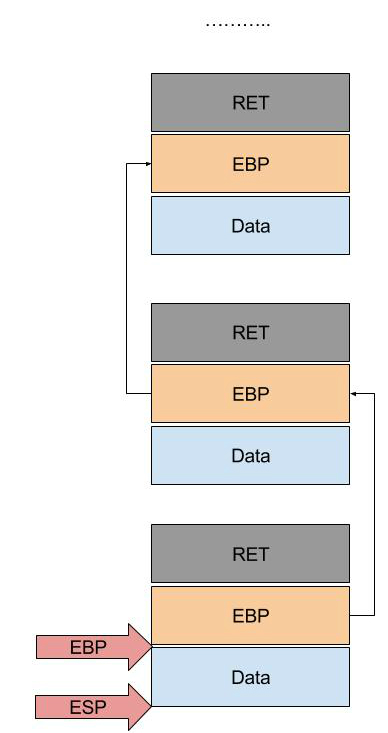
\includegraphics[scale=0.5]{images/call_stack}
    \end{figure}  
    
    Многие компиляторы при включении оптимизаций, например опцией \verb|-O2|, по умолчанию включает опцию \verb|-fomit-frame-pointer|, которая разрешает компилятору не сохранять в регистр EBP адрес на начало стекового кадра, для большей производительности. Из-за чего становится очень сложно получить стек вызовов. Поэтому большинство профайлеров требует от пользователей, чтобы они компилировали свои приложения, перед началом профилирования, с опцией \verb|-fno-omit-frame-pointer|, которая заставляет компилятор сохранять в регистр адрес на начало кадра.
    
    Сначала была написана своя функция по развертки стека вызовов, из-за простоты реализации и понимания происходящего. Но после было решено использовать библиотеку \verb|libunwind|. Она способна разматывать стек как с опцией сохранения EBP так и без него. Удается ей это сделать при помощи анализа отладочной информации хранящейся в бинарном файле. Однако по прежнему приложение желательно компилировать с опцией \verb|-fno-omit-frame-pointer| для более быстрого получения стека вызовов. Также наблюдались случаи, когда библиотека \verb|libunwind| неправильно разворачивала стек, если отсутствовала опция компилятора для сохранения информации о начале стекового кадра. В этой библиотеке присутствует возможность разворачивать стек удалено. Это можно делать только после того, как мы подключились к приложению и приостановили его работу.
        
\section{Сбор символов динамических библиотек}
	Динамическая библиотека сделана для загрузки в приложение во время запуска или во время исполнения, в отличии от статических которые нацелены, чтобы копироваться полностью в приложение, создавая монолитный исполняемый файл. Динамическая библиотека собирается с опцией компилятора \verb|-fPIC|, что создает независимый от размещения в памяти код. Все адреса функций в нем относительны, а не абсолютны, как это обычно бывает в бинарном файле. 
    
    \begin{figure}[H]
        \caption{Отображение динамических библиотек в приложении}
        \label{fig:dynamic_lib}
        \centering
        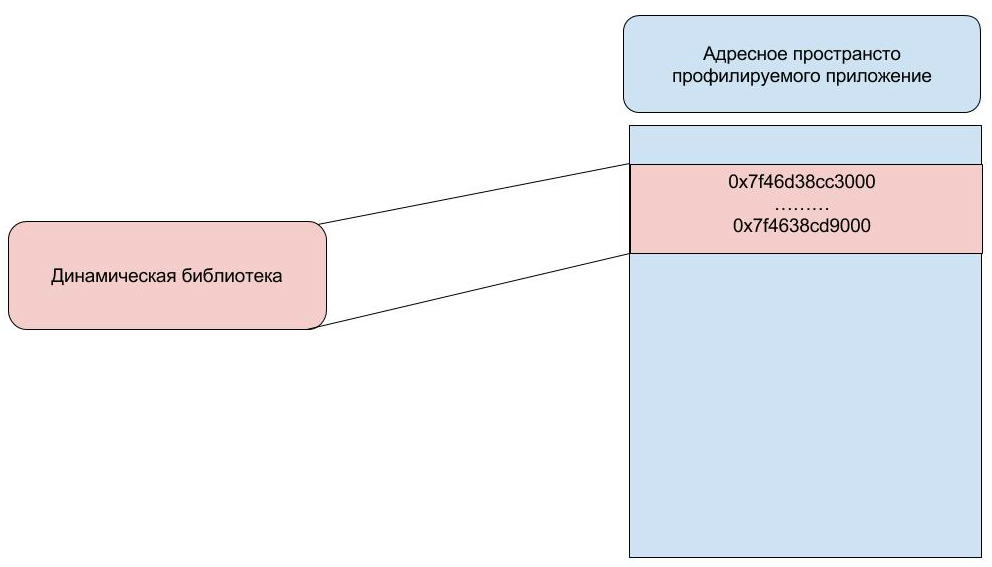
\includegraphics[width=\linewidth]{images/dynamic_lib}
    \end{figure} 
    
    Так как адреса функций в динамических библиотеках относительны, нужно узнать в каком диапазоне адресов была подгружена какая библиотека, пример на рисунке \ref{fig:dynamic_lib}. Эту информацию можно найти в файловой системе \verb|procfs|. В разделе \verb|/proc/pid/maps|. Пример строчки из этого файла:
\begin{lstlisting}
    7f46d38cc3000-7f4638cd9000  r-xp  ...  /lib/libc-2.23.so
\end{lstlisting}
    В ней можно увидеть в какой диапазон адресов загрузилась библиотека libc. Что она загрузилась на чтение и исполнение. После того как мы узнали по какому адресу находится библиотека, можно прочитав ее символы и относительные их адреса понять абсолютные адреса расположения объектов, которые будут подгружены в наше приложение.
    
    Для чтения символов исполняемого файла, использовалась утилита \verb|readelf|, которая может предоставить манглированные имена всех функций данного файла, адреса по которым они располагаются и размер в байтах который занимает функция. Изначально деманглирование символов происходило с помощью функции \verb|abi::__cxa_demangle(...)| предоставляемой библиотекой \verb|libstdc++|. Но в ходе работы было обнаружено, что деманглирование некоторых имен  с ее помощью работает неправильно. Так например если вызвать эту функции для вполне нормального имени функции \verb|g()|, то она его превратит в \verb|__float128()|. После этого было решено использовать утилиту \verb|c++filt| для деманглирования имен, которая не имеет такой проблемы. За время работы профайлера проблем с ней не возникло. Вся эта информация сохраняется в файл с собранными стеками вызовов перед завершением профилируемой программы, либо при получение сигнала \verb|SIGTERM|. 

    
\section{Скорость работы}
	Проводилось множество различных экспериментов и замеров накладных расходов профайлера на приложения. Одно из них представлено в листинге \ref{code:logger}. В программе работают два потока, один из них занимается тем, что берет данные из буфера и записывает их в файл, второй поток записывает данные в буфер и уведомляет второй, что появились новые данные. Эта программа интересна с точки зрения замеров профайлера в том плане, что в ней присутствует несколько потоков, а также большую часть времени она находится в блокировке под мьютексом. В ней производится множество запусков и считается среднее время. Измерения показали, что написанный профайлер замедляет данное приложение всего лишь на 3\%. Количество сэмплов было выставлено 100 в секунду, что вполне достаточно для показательного профиля в большинстве случаев. 
    
    Второе измерение производилось на программе представленной в \ref{code:writer}. На ней измерения показали ухудшений в производительности на 5\%. В сравнении с утилитой perf - она замедляла на 3\%.
    
    В процессе измерений было показано, что данный профайлер, хорошо справляется с поставленной задачей. Максимальное замедление, которое встречалось в процессе измерений было 10\%. 
        
\chapterconclusion
	В данной главе был описан алгоритм с помощью которого происходит сбор информации о профилируемом приложении. Были рассмотрены разные подходы и их проблемы к решению поставленной задачи. Были показаны замеры накладных расходов, накладываемых профайлером на приложение. В итоге был выбран наиболее подходящий алгоритм для сбора информации о запущенном приложении.
%-*-coding: utf-8-*-
\chapter{Визуализация собранной информации}
	В данной главе будут рассмотрены подходы к визуализации данных собранных профайлером. Существующие инструменты для визуализации их плюсы и недостатки. Также будет показано решение, которое было реализовано в ходе написания работы. 

\section{Обзор существующих средств для визуализации}
	Рассмотрим несколько самых популярных вариантов визуализации собранных данных профайлером:
    \begin{enumerate}
    	\item текстовый формат
        \item утилита KCachegrind
        \item огненная диаграмма (flame graph)
        \item граф вызовов
    \end{enumerate}

	Далее будут показаны плюсы и минусы этих подходов. Например \verb|gprof| осуществляет отображение профиля в текстовом формате, результат работы утилиты \verb|gprof| приведен в листинге \ref{lst:gprof}.
    
\begin{algorithm}[!h]
  \caption{Результат работы gprof}
  \label{lst:gprof}
  \begin{lstlisting}
    Each sample counts as 0.01 seconds.
      %   cumulative   self              
     time   seconds   seconds    name    
     60.25      0.03     0.03    foo()
     20.08      0.04     0.01    std::__cxx11::basic_string<...
     20.08      0.05     0.01    std::vector<std::__cxx11::...
      0.00      0.05     0.00    _GLOBAL__sub_I__Z10sighandleri
  \end{lstlisting}
\end{algorithm}

	Анализировать текстовый формат достаточно трудоемкое занятие. Возможность отсортировать по другому столбцу отсутствует. Благодаря большим сигнатурам функций очень сложно разглядеть из названия. Из этого представления мы можем сделать лишь вывод сколько времени занимала каждая из функций, но этой информации зачастую недостаточно. В большинстве случаев решающую роль играет где вызывали эту функцию, возможно стоит уменьшить количество ее вызовов. Но в таком формате данная информация теряется. 
    
    Из плюсов можно отметить, что текстовый формат очень прост в генерации, не требует дополнительных инструментов для анализа. Возможно его использовать без графической оболочки, что упрощает профилирование на удаленных машинах. Однако для того, чтобы найти узкие места, придется потратить много времени.
    
    Следующий кандидат для визуализации был инструмент kCacheGrind. Например программа valgrind визуализирует результат своей работы в специальном формате для отображения в kCacheGrind, пример приведен на рисунке \ref{fig:kCacheGrind}.
    
    \begin{figure}[H]
        \caption{визуализация с помощью kCacheGrind}
        \label{fig:kCacheGrind}
        \centering
        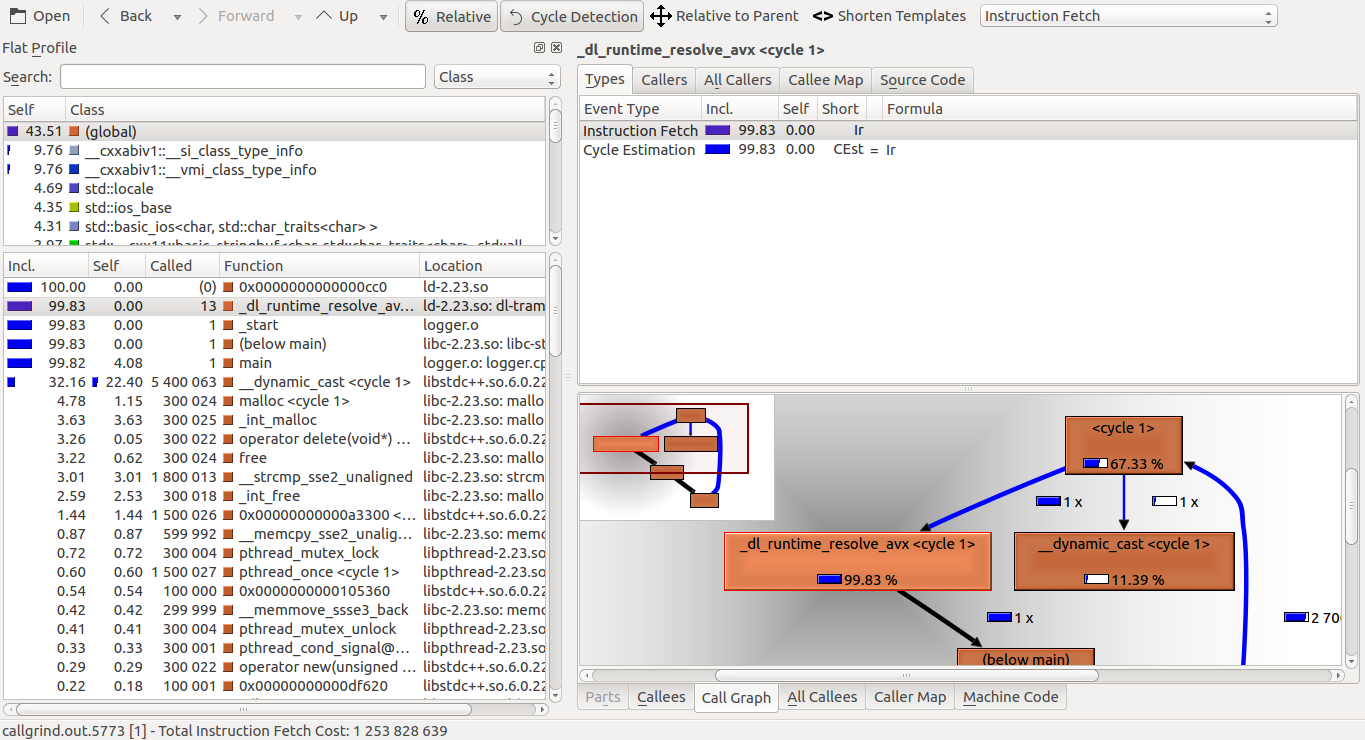
\includegraphics[scale=0.3]{images/kCacheGrind}
    \end{figure}
    
    Инструмент позволяет отображать собранную информацию в виде графа вызовов. С возможностью переходить к нужному методу по нажатию в вершине графа. Также есть возможность аннотировать исходный код с выделением горячих мест. Есть несколько режимов визуализации от вызываемого и от вызывающего.
    
    Недостатки данного инструмента заключается в сложности расширения функциональности. Формат входного файла представляет фиксированные структуры, для расширения которых нужно будет переделывать значительную часть инструмента. Также он очень громоздкий, что замедляет время работы и делает его более запутанным.
    
    Также была идея использовать огненная диаграмма \cite{flamegraph} для отображения собранной информации. Его можно построить после профилирования perf. Существует несколько скриптов которые преобразовывают файл perf.data в соответствующее отображение. Его преимущества в наглядности и простоте отображения. У него также есть возможность сужать профиль при нажатии на интересующую функцию, что делает его очень удобным для анализа профиля. Пример показан на рисунке \ref{fig:flamegraph}.
    
    \begin{figure}[H]
        \caption{визуализация с помощью огненной диаграммы}
        \label{fig:flamegraph}
        \centering
        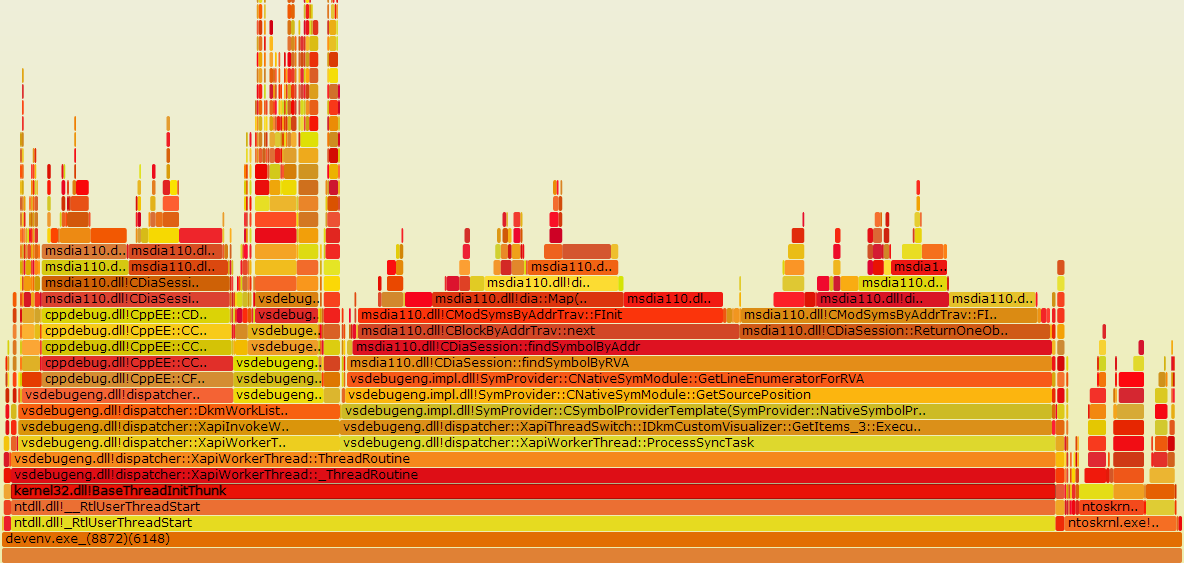
\includegraphics[scale=0.5]{images/flamegraph}
    \end{figure}
    
	Однако в таком отображении есть и свои недостатки. Его было бы сложно перерисовывать каждый раз при изменении времени. Так как это делается сторонней библиотекой. Пришлось бы каждый раз писать новый, суженный профиль в файл и вызывать соответствующий скрипт. После снова отображать его, что занимает значительную часть времени. В таком формате еще очень сложно выделить названия функций, когда сигнатура может быть очень длинной за счет использования шаблонов, что уменьшает видимость и акцент на функциях. Переписать заново библиотеку для создания огненных диаграмм было бы очень трудоемким и не оправданным решением.
    
    В компании Google при написании профайлера gperftools было решено визуализировать собранную информацию в виде графа вызовов. Красивое, наглядное и простое решение, пример можно увидеть на рисунке \ref{fig:callgraph}. Делают они это при помощи утилиты graphviz \cite{graphviz}. Главный минус такого подхода - когда есть большое разнообразие вызываемых функций очень сложно увидеть подходящую и весь граф мешает сосредоточится на нужных. 
	
    \begin{figure}[H]
        \caption{визуализация с помощью графа вызовов}
        \label{fig:callgraph}
        \centering
        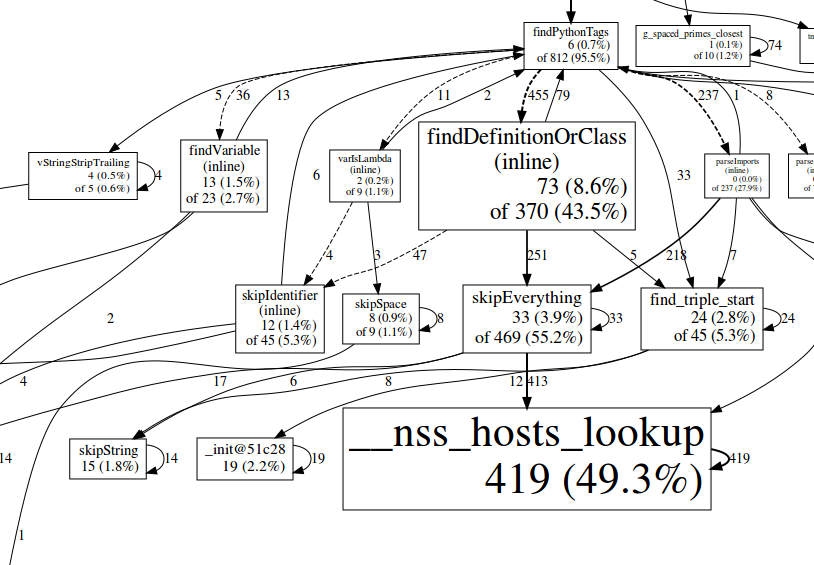
\includegraphics[scale=0.5]{images/callgraph}
    \end{figure}
    
\section{Разрешение символов}
	Программа для визуализации получает на вход файл \verb|pdb.data| - является результатом работы инструмента по сбору информацию, содержащий все стеки вызовов потоков за время профилирования. Символы библиотек загруженных на тот момент. Также символы самого исполняемого файла, которое было профилировано. Сохранение всех символов в файл необходимо для разрешения адресов на другой машине. Так как библиотеки и их версии могут сильно отличаться на другом компьютере, то без них нельзя узнать названия объектов расположенных по определенным адресам. Это позволяет профилировать приложения на удаленном компьютере, а после анализировать профиль локально. 
    
    Для каждого стека вызовов известны адреса, которые были получены при помощи библиотеки \verb|libunwind|. Эти адреса представляют из себя \enquote{позицию} в функции, на тот момент, когда программа была приостановлена профайлером. Необходимо из этих адресов понять к какой функции они относятся, т.к. из инструмента по сбору была получена информация только про начала функций и их размер. Когда мы смогли преобразовать изначальные адреса в адреса начал функций, можно строить дерево для отображения всей информации.
    
    По преобразованным адресам на начало функций строится два дерева. В каждой вершине дерева считается количество вызовов проходящих через нее. Процент времени, который программа провела в данной функции считается как количество сэмплов которые попали на данную функцию деленное на общее количество сэмплов. Далее адреса преобразуются в деманглированные имена функций и отображаются в визуализаторе.

\section{Режимы отображения собранной информации}
	В инструменте для визуализации можно менять режимы отображения стеков вызовов для более детального анализа профиля приложения. Существует два наиболее распространенных режима для отображения собранных данных:
    \begin{enumerate}
    	\item от вызывающего к вызываемому
        \item от вызываемого к вызывающему
    \end{enumerate}
    
    Оба этих подхода полезны при поиске \enquote{узких} мест в приложениях и анализе профиля. Вид от вызывающего к вызываемому полезен когда необходимо понимать какую долю времени занимает каждая дочерняя функция внутри вызывающего. Также данный подход хорошо отображает все функции которые были вызваны из каждой, что помогает глубже понять работу программы. Пример отображения информации с помощью этого подхода показан на рис. \ref{fig:top-down}, полученный отчет после профилирования программы написанной в листинге \ref{code:prof_top_down}. На нем отчетливо видно какие функции вызывались из \verb|main()| также отображено, что \verb|foo()| и \verb|bar()| занимают примерно одинаковое время работы.
    
    Второй подход от вызываемого к вызывающему отличается от предыдущего. Здесь информация о всех стеках вызовах разворачивается в другую сторону. Этот подход помогает при поиске функций, которые сами по себе занимают не очень много времени, но их очень часто используют другие, что может привести к замедлению программы. Также данный подход показывает всё разнообразие функций, которые используются в приложении. Пример такого отображения показан на рис. \ref{fig:down-top}. На нем видно, что функция \verb|f()| вызывалась из функций \verb|foo()| и \verb|bar()| также, что она занимала все 100\% времени работы.

    \begin{algorithm}[!h]
      \caption{Пример профилируемой программы}\label{code:prof_top_down}
      \begin{lstlisting}
          #include <unistd.h>
          int f() { 
              sleep(1); 
              return 42; 
          }
          int foo() { 
              return f(); 
          }
          int bar() { 
              return f(); 
          }
          int main() {
              foo();
              bar();
          }
      \end{lstlisting}
	\end{algorithm}    
    
    \begin{figure}[H]
        \caption{профиль от вызывающего к вызываемому}
        \label{fig:top-down}
        \centering
        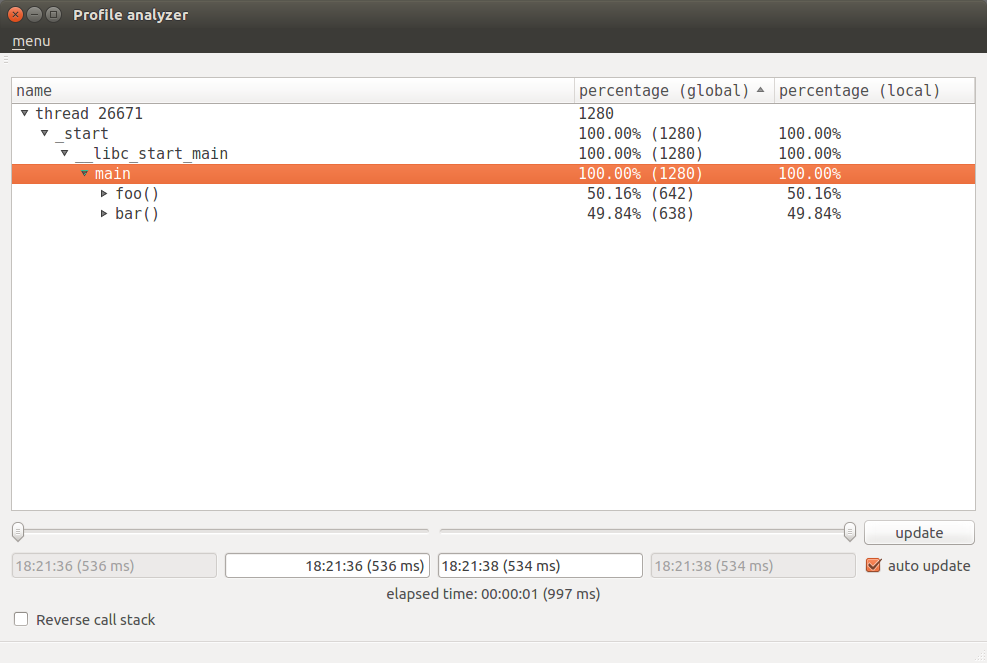
\includegraphics[scale=0.47]{images/top-down}
    \end{figure}    
        
    \begin{figure}[H]
        \caption{профиль от вызываемого к вызывающему}
        \label{fig:down-top}
        \centeringы
        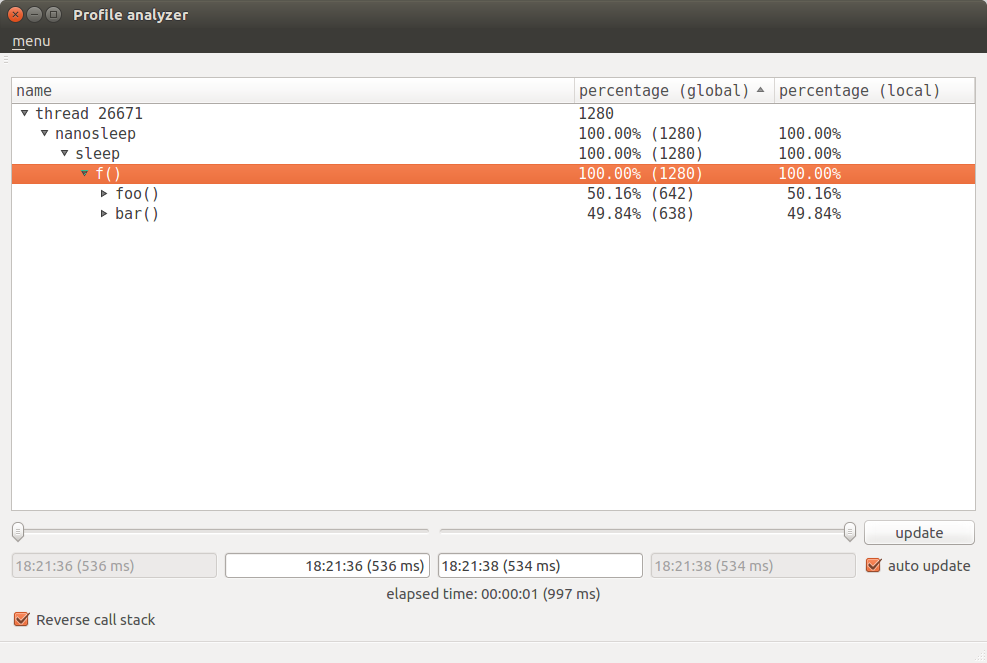
\includegraphics[scale=0.47]{images/down-top}
    \end{figure}
    

\section{Отображение для конкретного временного промежутка}
	Для инструмента отображающего собранные данные необходимо было реализовать возможность для сужения профиля на определенные временные промежутки. Данная функция была реализована при помощи двух ползунков, при изменении которых пересчитывались деревья вызовов. Один из них изменяет время левой границы т.е. начало профилирования, а второй время правой.
    
    При изменении ползунков производится проход по обоим деревьям и пересчитываются сэмплы которые были собранны в данных временных промежутках. Каждая вершина хранит вектор временных меток - сэмплы которые были сделаны и закончились в этой вершине. После бинарным поиском находятся границы соответствующие заданным пользователем. Данные пересчитываются и информация об обновленном количестве сэмплов передается родителю от ребенка. Таким образом получаем дерево с пересчитанными значениями.
    
    После того как были получены новые значения, производится скрытие тех вершин в графическом интерфейсе у которых размер сэмплов стал равен нулю. Таким образом в процессе изменения слайдеров могут появляться и исчезать вершины дерева, отображенного на графическом интерфейсе. Таким образом данный алгоритм работает в худшем случае за количество сэмплов собранных профайлером, а в лучшем за логарифм от их количества. 
    
\section{Выделение имени функции}
	В процессе работы с графическим инструментом было решено выделять имена функций, так как они сливаются в сигнатуре и их сложно увидеть. Был реализован алгоритм для выделения имени из сигнатуры.
    
    После нахождения имени, сигнатура делится на три части: пространство в котором находится данная функция, ее имя, аргументы. Возвращаемый тип не указывается, так как он отсутствует в символьной информации бинарного файла. Для виджета \verb|QTreeWidget| был переопределен делегат, который рисует черным цветом первую часть, выделяет синим имя функции, и дорисовывает оставшуюся часть. 
    
    Функции которые занимают меньше одного процента выделяются серым цветом, чтобы не отвлекать внимание пользователя. Для них тоже происходит подсветка имени, только темно серым цветом результат можно увидеть на рисунке \ref{fig:highlighting}
    \begin{figure}[H]
        \caption{выделение имен функций}
        \label{fig:highlighting}
        \centering
        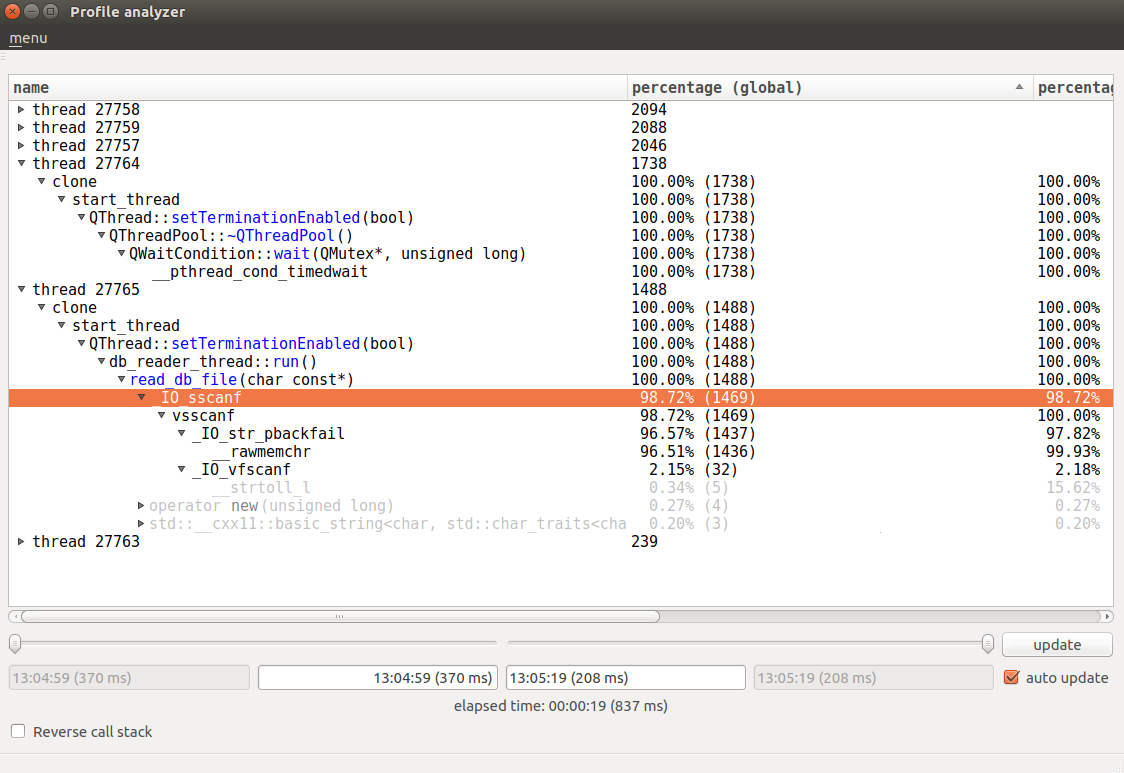
\includegraphics[scale=0.35]{images/highlighting}
    \end{figure}	
    
\chapterconclusion
	В данной главе было рассказано про существующие инструменты для отображения собранной информации. Показаны их недостатки, почему выбор был сделан именно таким. Рассказаны внутренние детали реализации графического интерфейса. 

% %-*-coding: utf-8-*-
\chapter{Таблицы}

В качестве примера таблицы приведена таблица~\ref{tab1}.

\begin{table}[!h]
\caption{Таблица умножения (фрагмент)}\label{tab1}
\centering
\begin{tabular}{|*{18}{c|}}\hline
-- & 1 & 2 & 3 & 4 & 5 & 6 & 7 & 8 & 9 & 10 & 11 & 12 & 13 & 14 & 15 & 16 & 17 \\\hline
1  & 1 & 2 & 3 & 4 & 5 & 6 & 7 & 8 & 9 & 10 & 11 & 12 & 13 & 14 & 15 & 16 & 17 \\\hline
2  & 2 & 4 & 6 & 8 & 10 & 12 & 14 & 16 & 18 & 20 & 22 & 24 & 26 & 28 & 30 & 32 & 34 \\\hline
3  & 3 & 6 & 9 & 12 & 15 & 18 & 21 & 24 & 27 & 30 & 33 & 36 & 39 & 42 & 45 & 48 & 51 \\\hline
4  & 4 & 8 & 12 & 16 & 20 & 24 & 28 & 32 & 36 & 40 & 44 & 48 & 52 & 56 & 60 & 64 & 68 \\\hline
\end{tabular}
\end{table}

Есть еще такое окружение \texttt{tabu}, его можно аккуратно растянуть на всю страницу.
Приведем пример (таблица~\ref{tab2}).

\begin{table}[!h]
\caption{Таблица умножения с помощью \texttt{tabu} (фрагмент)}\label{tab2}
\centering
\begin{tabu}{|*{18}{X[c]|}}\hline
-- & 1 & 2 & 3 & 4 & 5 & 6 & 7 & 8 & 9 & 10 & 11 & 12 & 13 & 14 & 15 & 16 & 17 \\\hline
1  & 1 & 2 & 3 & 4 & 5 & 6 & 7 & 8 & 9 & 10 & 11 & 12 & 13 & 14 & 15 & 16 & 17 \\\hline
2  & 2 & 4 & 6 & 8 & 10 & 12 & 14 & 16 & 18 & 20 & 22 & 24 & 26 & 28 & 30 & 32 & 34 \\\hline
3  & 3 & 6 & 9 & 12 & 15 & 18 & 21 & 24 & 27 & 30 & 33 & 36 & 39 & 42 & 45 & 48 & 51 \\\hline
4  & 4 & 8 & 12 & 16 & 20 & 24 & 28 & 32 & 36 & 40 & 44 & 48 & 52 & 56 & 60 & 64 & 68 \\\hline
\end{tabu}
\end{table}

\section{Рисунки}

Пример рисунка (c помощью \texttt{TikZ}) приведен на рисунке~\ref{fig1}. Под \texttt{pdflatex} можно также
использовать \texttt{*.jpg}, \texttt{*.png} и даже \texttt{*.pdf}, под \texttt{latex} можно использовать
Metapost. Последний можно использовать и под \texttt{pdflatex}, для чего в стилевике продекларированы
номера картинок от~1 до~20.

\begin{figure}[!h]
\caption{Пример рисунка}\label{fig1}
\centering
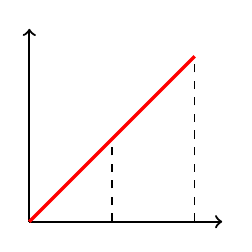
\begin{tikzpicture}[scale=0.7]
\draw[thick,->] (0,0)--(3.5,0);
\draw[thick,->] (0,0)--(0,3.5);
\draw[very thick, red] (0,0)--(3,3);
\draw[dashed] (3,0)--(3,3);
\draw[dashed] (1.5,0)--(1.5,1.5);
\end{tikzpicture}
\end{figure}

\section{Листинги}

В работах студентов кафедры <<Компьютерные технологии>> часто встречаются листинги. Листинги бывают
двух основных видов~--- исходный код и псевдокод. Первый оформляется с помощью окружения \texttt{lstlisting}
из пакета \texttt{listings}, который уже включается в стилевике и немного настроен. Пример Hello World на Java
приведен на листинге~\ref{lst1}.

\begin{lstlisting}[float=!h,caption={Пример исходного кода на Java},label={lst1}]
public class HelloWorld {
	public static void main(String[] args) {
		System.out.println("Hello, world!");
	}
}
\end{lstlisting}

Псевдокод можно оформлять с помощью разных пакетов. В данном стилевике включается пакет \texttt{algorithmicx}.
Сам по себе он не генерирует флоатов, поэтому для них используется пакет \texttt{algorithm}.
Пример их совместного использования приведен на листинге~\ref{lst2}. Обратите внимание, что флоаты разные, а 
нумерация~--- общая!

\begin{algorithm}[!h]
\caption{Пример псевдокода}\label{lst2}
\begin{algorithmic}
	\Function{IsPrime}{$N$}
		\For{$t \gets [2; \lfloor\sqrt{N}\rfloor]$}
			\If{$N \bmod t = 0$}
				\State\Return \textsc{false}
			\EndIf
		\EndFor
		\State\Return \textsc{true}
	\EndFunction
\end{algorithmic}
\end{algorithm}

Наконец, листинги из \texttt{listings} тоже можно подвешивать с помощью \texttt{algorithm},
пример на листинге~\ref{lst3}.

\begin{algorithm}[!h]
\caption{Исходный код и флоат \texttt{algorithm}}\label{lst3}
\begin{lstlisting}
public class HelloWorld {
	public static void main(String[] args) {
		System.out.println("Hello, world!");
	}
}
\end{lstlisting}
\end{algorithm}

\chapter{Проверка сквозной нумерации}

Листинг~\ref{lst4} должен иметь номер 4.

\begin{algorithm}[!h]
\caption{Исходный код и флоат \texttt{algorithm}}\label{lst4}
\begin{lstlisting}
public class HelloWorld {
	public static void main(String[] args) {
		System.out.println("Hello, world!");
	}
}
\end{lstlisting}
\end{algorithm}

Рисунок~\ref{fig2} должен иметь номер 2.

\begin{figure}[!h]
\caption{Пример рисунка}\label{fig2}
\centering
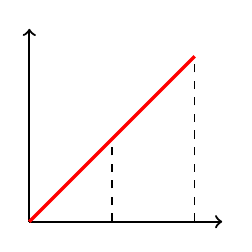
\begin{tikzpicture}[scale=0.7]
\draw[thick,->] (0,0)--(3.5,0);
\draw[thick,->] (0,0)--(0,3.5);
\draw[very thick, red] (0,0)--(3,3);
\draw[dashed] (3,0)--(3,3);
\draw[dashed] (1.5,0)--(1.5,1.5);
\end{tikzpicture}
\end{figure}

Таблица~\ref{tab3} должна иметь номер 3.

\begin{table}[!h]
\caption{Таблица умножения с помощью \texttt{tabu} (фрагмент)}\label{tab3}
\centering
\begin{tabu}{|*{18}{X[c]|}}\hline
-- & 1 & 2 & 3 & 4 & 5 & 6 & 7 & 8 & 9 & 10 & 11 & 12 & 13 & 14 & 15 & 16 & 17 \\\hline
1  & 1 & 2 & 3 & 4 & 5 & 6 & 7 & 8 & 9 & 10 & 11 & 12 & 13 & 14 & 15 & 16 & 17 \\\hline
2  & 2 & 4 & 6 & 8 & 10 & 12 & 14 & 16 & 18 & 20 & 22 & 24 & 26 & 28 & 30 & 32 & 34 \\\hline
3  & 3 & 6 & 9 & 12 & 15 & 18 & 21 & 24 & 27 & 30 & 33 & 36 & 39 & 42 & 45 & 48 & 51 \\\hline
4  & 4 & 8 & 12 & 16 & 20 & 24 & 28 & 32 & 36 & 40 & 44 & 48 & 52 & 56 & 60 & 64 & 68 \\\hline
\end{tabu}
\end{table}

\chapterconclusion

В конце каждой главы желательно делать выводы. Вывод по данной главе~--- нумерация работает корректно, ура!


% -*-coding: utf-8-*-

\startconclusionpage
	Описанные инструменты в данной работе были успешно реализованы и использованы в компании ООО «Научно-Технический Центр ПРОТЕЙ». Применился в проекте GGSN \cite{ggsn}, одной из его функций является маршрутизацией пользовательского трафика. Для каждого абонента заводились различные таймера, по истечении которых происходили определенные действия: например запрос на удаление пользователя (DELETE PDP CONTEXT REQUEST), либо отправление запроса на обновление используемых данных в RADIUS \cite{radius} сервер. Так как абонентов большое количество, требовалась реализация таймеров с высокой производительностью. Таймеры были взяты из набора библиотек DPDK \cite{dpdk}, они реализованы с помощью структуры данных - список с пропусками \cite{skip_list}. При тестировании проекта были обнаружены замедления. Благодаря написанному профайлеру стало известно, что замедление происходило из-за таймеров. На рисунке \ref{fig:slow_timers_profile} показан профиль приложения, в котором была вынесена отдельная работа с таймерами.
    \begin{figure}[H]
        \caption{профиль приложения работающего с таймерами из DPDK}
        \label{fig:slow_timers_profile}
        \centering
        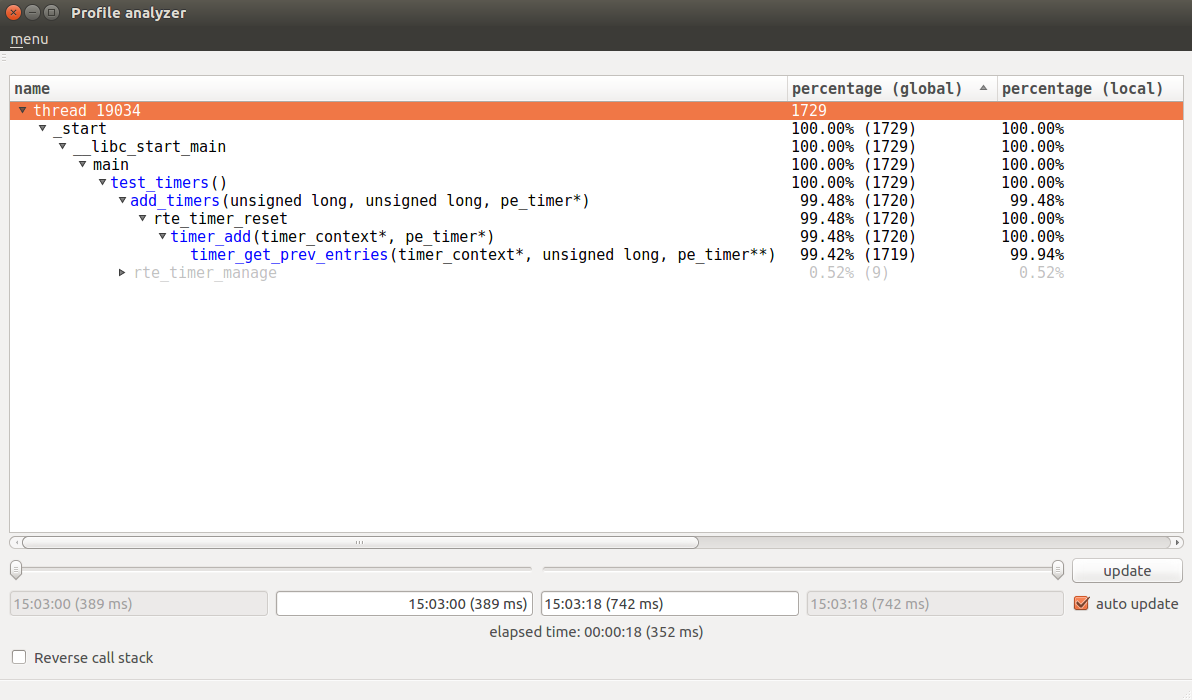
\includegraphics[scale=0.4]{images/slow_timers_profile}
    \end{figure}    
    
    Из профиля видно, что большую часть времени занимает добавление нового таймера. Хотя добавление имеет такую же сложность как и функция поиска истекших таймеров (на рисунке это \verb|rte_timer_manage|). При дальнейшем анализе обнаружилась ошибка в библиотеке, которая возникала из-за удаления ссылок на старших уровнях списка с пропусками, при срабатывании таймера который не был расположен на них. Из-за этого асимптотика работы добавления таймера  начинала занимать $O($количества добавленных таймеров$)$, т.е. сложность была линейной, а не логарифмической. Исправление ошибки заметно ускорило приложение.    
    
    Написанный профайлер также успешно использовался при оптимизации себя же. Благодаря ему были выявлены узкие места в инструменте для визуализации данных, исправление которых ускорило его. Проблема была в использовании функции \verb|sscanf| при считывании символов записанных в файл после работы инструмента по сбору данных. Оказалось, что она внутри вызывает подобие \verb|strlen| которая считает длину буфера, пробегая по нему в поисках \verb|\0|. В файле было записано много строк, содержащих адрес на начало функции, размер ее и имя функции. После прочтения одной строчки, указатель на начало буфера сдвигался на размер строки и разбор файла продолжался дальше. Так как такая строчка занимает не больше 1000 символов, то \verb|sscanf| вызывался $O($размера буффера$)$ раз. В итоге получилось, что функция разбора символов работала за $O(($размер буффера$) ^ 2)$. Замена \verb|sscanf| на самописную функцию дало ускорение, т.е. разбор файла стал работать за $O($размер буффера$)$. Также был оптимизирован инструмент для сбора информации, в котором происходило постоянное сбрасывание буфера при создании файла с данными, что было обнаружено благодаря написанному профайлеру. %% Успешно применился и помог ускорить решения написанные в нашей компании.
    
    В дальнейшем планируется добавить возможность профилировать в реальном времени. Для этого нужен будет агент, который будет запускаться на удаленной машине, с возможность подключения к нему. Также планируется расширить его с добавлением возможности визуализировать пользовательские данные в зависимости от времени. Еще остается вопрос производительности, планируется уменьшить накладные расходы профайлера на приложение.
	

\printmainbibliography

%% После этой команды chapter будет генерировать приложения, нумерованные русскими буквами.
%% \startappendices из старого стилевика будет делать то же самое
\appendix

\chapter{Измерение времени работы}

Здесь будут показаны несколько различных программ на которых проводилось исследование накладных расходов,  появляющихся в результате работы профайлера.

\lstinputlisting[label=code:logger,caption=Исходный код программы для логирования]{appendix/logger.tex}

\lstinputlisting[label=code:writer,caption=Исходный код программы записывающей различные значения]{appendix/writer.tex}

























% В приложениях рисунки, таблицы и другие подобные элементы нумеруются по приложениям с соответствующим префиксом. Проверим это.

% Листинг~\ref{lst4:apx} должен иметь номер А.1.

% \begin{algorithm}[!h]
% \caption{Исходный код и флоат \texttt{algorithm}}\label{lst4:apx}
% \begin{lstlisting}
% public class HelloWorld {
% 	public static void main(String[] args) {
% 		System.out.println("Hello, world!");
% 	}
% }
% \end{lstlisting}
% \end{algorithm}

% Рисунок~\ref{fig2:apx} должен иметь номер A.1.

% \begin{figure}[!h]
% \caption{Пример рисунка}\label{fig2:apx}
% \centering
% \begin{tikzpicture}[scale=0.7]
% \draw[thick,->] (0,0)--(3.5,0);
% \draw[thick,->] (0,0)--(0,3.5);
% \draw[very thick, red] (0,0)--(3,3);
% \draw[dashed] (3,0)--(3,3);
% \draw[dashed] (1.5,0)--(1.5,1.5);
% \end{tikzpicture}
% \end{figure}

% Таблица~\ref{tab3:apx} должна иметь номер A.1.

% \begin{table}[!h]
% \caption{Таблица умножения с помощью \texttt{tabu} (фрагмент)}\label{tab3:apx}
% \centering
% \begin{tabu}{|*{18}{X[c]|}}\hline
% -- & 1 & 2 & 3 & 4 & 5 & 6 & 7 & 8 & 9 & 10 & 11 & 12 & 13 & 14 & 15 & 16 & 17 \\\hline
% 1  & 1 & 2 & 3 & 4 & 5 & 6 & 7 & 8 & 9 & 10 & 11 & 12 & 13 & 14 & 15 & 16 & 17 \\\hline
% 2  & 2 & 4 & 6 & 8 & 10 & 12 & 14 & 16 & 18 & 20 & 22 & 24 & 26 & 28 & 30 & 32 & 34 \\\hline
% 3  & 3 & 6 & 9 & 12 & 15 & 18 & 21 & 24 & 27 & 30 & 33 & 36 & 39 & 42 & 45 & 48 & 51 \\\hline
% 4  & 4 & 8 & 12 & 16 & 20 & 24 & 28 & 32 & 36 & 40 & 44 & 48 & 52 & 56 & 60 & 64 & 68 \\\hline
% \end{tabu}
% \end{table}

% Заодно проверим нумерованные и ненумерованные перечисления. Ненумерованные:
% \begin{itemize}
%     \item пункт А;
%     \item пункт Б;
%     \item пункт В.
% \end{itemize}

% Нумерованные списки нескольких уровней:
% \begin{enumerate}
%     \item первый элемент;
%     \item второй элемент с подэлементами:
%     \begin{enumerate}
%         \item первый подэлемент;
%         \item второй подэлемент;
%         \item третий подэлемент.
%     \end{enumerate}
%     \item третий элемент;
%     \item четвертый элемент;
%     \item пятый элемент;
%     \item шестой элемент;
%     \item седьмой элемент;
%     \item восьмой элемент;
%     \item девятый элемент;
%     \item десятый элемент.
% \end{enumerate}

% \chapter{Еще один пример приложения  с неимоверно длиннющим названием для тестирования переносов}

% Проверим на примере таблиц, что нумерация в приложениях~--- по приложениям.
% Таблица~\ref{tab3:apx2} должна иметь номер Б.1.

% \begin{table}[!h]
% \caption{Таблица умножения с помощью \texttt{tabu} (фрагмент)}\label{tab3:apx2}
% \centering
% \begin{tabu}{|*{18}{X[c]|}}\hline
% -- & 1 & 2 & 3 & 4 & 5 & 6 & 7 & 8 & 9 & 10 & 11 & 12 & 13 & 14 & 15 & 16 & 17 \\\hline
% 1  & 1 & 2 & 3 & 4 & 5 & 6 & 7 & 8 & 9 & 10 & 11 & 12 & 13 & 14 & 15 & 16 & 17 \\\hline
% 2  & 2 & 4 & 6 & 8 & 10 & 12 & 14 & 16 & 18 & 20 & 22 & 24 & 26 & 28 & 30 & 32 & 34 \\\hline
% 3  & 3 & 6 & 9 & 12 & 15 & 18 & 21 & 24 & 27 & 30 & 33 & 36 & 39 & 42 & 45 & 48 & 51 \\\hline
% 4  & 4 & 8 & 12 & 16 & 20 & 24 & 28 & 32 & 36 & 40 & 44 & 48 & 52 & 56 & 60 & 64 & 68 \\\hline
% \end{tabu}
% \end{table}


\end{document}